\documentclass[]{article}

\usepackage[T1]{fontenc}
\usepackage[utf8]{inputenc}
\usepackage{amsthm, amsmath, amsfonts}
\usepackage{blkarray}
\usepackage{bigstrut}
\usepackage{graphicx}

\newcommand{\avaliacao}{2}
\newcommand{\disciplina}{Probabilidade e Estatística}
\newcommand{\semestre}{2024/1}


\theoremstyle{definition}
\newtheorem{ex}{Exercício}

\renewcommand{\SS}{\mathcal{S}}

\begin{document}
\thispagestyle{empty}
\begin{center}
\Large{\avaliacao ª Avaliação de \disciplina\ - \semestre}

\large{Prof. Dr. Alessandro José Queiroz Sarnaglia}
\end{center}

\begin{ex}
Suponha que apenas 35\% de todos os motoristas parem completamente num cruzamento com semáforo vermelho quando não há outros carros à vista.
\begin{enumerate}
	\item Se 10 motoristas são observados, qual a probabilidade de exatamente a metade parar completamente?
	\item Se 10 motoristas são observados, qual a probabilidade de ao menos a metade parar totalmente?
	\item Se fossem 100 motoristas, qual a probabilidade aproximada de ao menos a metade parar completamente?
\end{enumerate}
\end{ex}


\begin{ex}
O número $X$ de pessoas que chegam por hora para tratamento em um pronto-socorro é modelado por uma distribuição Poisson com média de três por hora.
\begin{enumerate}
	\item Qual é a probabilidade de três pessoas chegarem em certa hora?
	\item Qual é a probabilidade de ao menos três pessoas chegarem em certa hora?
\end{enumerate}
\end{ex}


\begin{ex}
O tempo $X$ de falha (em horas) de isolantes sólidos segue distribuição Weibull com $\alpha = 0.5$ e $\beta = 100$.
\begin{enumerate}
	\item Em média, quanto tempo leva para uma falha ocorrer?
	\item Que valor faz com que 50\% de todas as amostras tenham tempos de vida que excedam o valor?
\end{enumerate}
\end{ex}

\begin{ex}
Determinado evento ocorre em um ponto $(X,Y)$ na região ilustrada abaixo. Suponha que nenhum ponto é privilegiado para a ocorrência do evento.
\begin{enumerate}
	\item Encontre as fdp's marginais de $X$ e $Y$.
	\item Encontre $\text{Cov}(X,Y)$.
	\item As vac's $X$ e $Y$ são independentes? Justifique!
\end{enumerate}
\begin{center}
	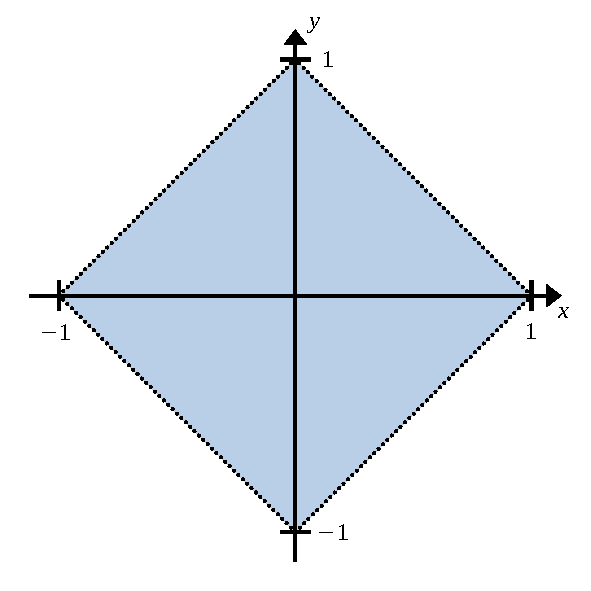
\includegraphics[width=0.45\linewidth]{figura}
\end{center}
\end{ex}


\end{document}
